% Created 2019-02-01 ven. 20:30
% Intended LaTeX compiler: pdflatex
\documentclass[letterpaper,12pt, french]{article}
\usepackage[top=2.5cm]{geometry}
\usepackage[utf8]{inputenc}
\usepackage[T1]{fontenc}
\usepackage{babel}
\usepackage{graphicx}
\usepackage{grffile}
\usepackage{longtable}
\usepackage{wrapfig}
\usepackage{rotating}
\usepackage[normalem]{ulem}
\usepackage{amsmath}
\usepackage{textcomp}
\usepackage{amssymb}
\usepackage{fancyhdr}
\usepackage{capt-of}
\usepackage{hyperref}
\usepackage{verbatim}
\usepackage{minted}
\usepackage[T1]{fontenc}
\usepackage{hyperref}
\usepackage{subcaption}
\usepackage{enumitem}
\usepackage{listings}
\makeatother
\usepackage{xcolor}
\definecolor{default-linkcolor}{HTML}{A50000}
\definecolor{default-filecolor}{HTML}{A50000}
\definecolor{default-citecolor}{HTML}{4077C0}
\definecolor{default-urlcolor}{HTML}{4077C0}
\usepackage{titlesec}
\usepackage{tocloft}
\renewcommand{\cftaftertoctitle}{\hrulefill}

\usepackage[utf8]{inputenc}
\usepackage[english]{babel}
\usepackage{biblatex}
\addbibresource{sources/citations.bib}

%
%
% Listings
%
%


%
% general listing colors
%
\definecolor{listing-background}{HTML}{F7F7F7}
\definecolor{listing-rule}{HTML}{B3B2B3}
\definecolor{listing-numbers}{HTML}{B3B2B3}
\definecolor{listing-text-color}{HTML}{000000}
\definecolor{listing-keyword}{HTML}{435489}
\definecolor{listing-keyword-2}{HTML}{1284CA} % additional keywords
\definecolor{listing-keyword-3}{HTML}{9137CB} % additional keywords
\definecolor{listing-identifier}{HTML}{435489}
\definecolor{listing-string}{HTML}{00999A}
\definecolor{listing-comment}{HTML}{8E8E8E}

\lstdefinestyle{eisvogel_listing_style}{
  language         = java,
  numbers          = left,
  xleftmargin      = 2.7em,
  framexleftmargin = 2.5em,
  backgroundcolor  = \color{listing-background},
  basicstyle       = \color{listing-text-color}\linespread{1.0}\small\ttfamily{},
  breaklines       = true,
  frame            = single,
  framesep         = 0.19em,
  rulecolor        = \color{listing-rule},
  frameround       = ffff,
  tabsize          = 4,
  numberstyle      = \color{listing-numbers},
  aboveskip        = 1.0em,
  belowskip        = 0.1em,
  abovecaptionskip = 0em,
  belowcaptionskip = 1.0em,
  keywordstyle     = {\color{listing-keyword}\bfseries},
  keywordstyle     = {[2]\color{listing-keyword-2}\bfseries},
  keywordstyle     = {[3]\color{listing-keyword-3}\bfseries\itshape},
  sensitive        = true,
  identifierstyle  = \color{listing-identifier},
  commentstyle     = \color{listing-comment},
  stringstyle      = \color{listing-string},
  showstringspaces = false,
  escapeinside     = {/*@}{@*/}, % Allow LaTeX inside these special comments
  literate         =
  {á}{{\'a}}1 {é}{{\'e}}1 {í}{{\'i}}1 {ó}{{\'o}}1 {ú}{{\'u}}1
  {Á}{{\'A}}1 {É}{{\'E}}1 {Í}{{\'I}}1 {Ó}{{\'O}}1 {Ú}{{\'U}}1
  {à}{{\`a}}1 {è}{{\'e}}1 {ì}{{\`i}}1 {ò}{{\`o}}1 {ù}{{\`u}}1
  {À}{{\`A}}1 {È}{{\'E}}1 {Ì}{{\`I}}1 {Ò}{{\`O}}1 {Ù}{{\`U}}1
  {ä}{{\"a}}1 {ë}{{\"e}}1 {ï}{{\"i}}1 {ö}{{\"o}}1 {ü}{{\"u}}1
  {Ä}{{\"A}}1 {Ë}{{\"E}}1 {Ï}{{\"I}}1 {Ö}{{\"O}}1 {Ü}{{\"U}}1
  {â}{{\^a}}1 {ê}{{\^e}}1 {î}{{\^i}}1 {ô}{{\^o}}1 {û}{{\^u}}1
  {Â}{{\^A}}1 {Ê}{{\^E}}1 {Î}{{\^I}}1 {Ô}{{\^O}}1 {Û}{{\^U}}1
  {œ}{{\oe}}1 {Œ}{{\OE}}1 {æ}{{\ae}}1 {Æ}{{\AE}}1 {ß}{{\ss}}1
  {ç}{{\c c}}1 {Ç}{{\c C}}1 {ø}{{\o}}1 {å}{{\r a}}1 {Å}{{\r A}}1
  {€}{{\EUR}}1 {£}{{\pounds}}1 {«}{{\guillemotleft}}1
  {»}{{\guillemotright}}1 {ñ}{{\~n}}1 {Ñ}{{\~N}}1 {¿}{{?`}}1
  {…}{{\ldots}}1 {≥}{{>=}}1 {≤}{{<=}}1 {„}{{\glqq}}1 {“}{{\grqq}}1
  {”}{{''}}1
}
\lstset{style=eisvogel_listing_style}

%
% Java (Java SE 12, 2019-06-22)
%
\lstdefinelanguage{Java}{
  morekeywords={
    % normal keywords (without data types)
    abstract,assert,break,case,catch,class,continue,default,
    do,else,enum,exports,extends,final,finally,for,if,implements,
    import,instanceof,interface,module,native,new,package,private,
    protected,public,requires,return,static,strictfp,super,switch,
    synchronized,this,throw,throws,transient,try,volatile,while,
    % var is an identifier
    var
  },
  morekeywords={[2] % data types
    % primitive data types
    boolean,byte,char,double,float,int,long,short,
    % String
    String,
    % primitive wrapper types
    Boolean,Byte,Character,Double,Float,Integer,Long,Short
    % number types
    Number,AtomicInteger,AtomicLong,BigDecimal,BigInteger,DoubleAccumulator,DoubleAdder,LongAccumulator,LongAdder,Short,
    % other
    Object,Void,void
  },
  morekeywords={[3] % literals
    % reserved words for literal values
    null,true,false,
  },
  sensitive,
  morecomment  = [l]//,
  morecomment  = [s]{/*}{*/},
  morecomment  = [s]{/**}{*/},
  morestring   = [b]",
  morestring   = [b]',
}

\lstdefinelanguage{XML}{
  morestring      = [b]",
  moredelim       = [s][\bfseries\color{listing-keyword}]{<}{\ },
  moredelim       = [s][\bfseries\color{listing-keyword}]{</}{>},
  moredelim       = [l][\bfseries\color{listing-keyword}]{/>},
  moredelim       = [l][\bfseries\color{listing-keyword}]{>},
  morecomment     = [s]{<?}{?>},
  morecomment     = [s]{<!--}{-->},
  commentstyle    = \color{listing-comment},
  stringstyle     = \color{listing-string},
  identifierstyle = \color{listing-identifier}
}

\hypersetup{
    colorlinks=true,
    linkcolor=blue,
    filecolor=magenta,      
    urlcolor=blue,
}
\urlstyle{same}
\usepackage{tabularx}
\usepackage[letterpaper, portrait, lmargin=1in, rmargin=1in, bmargin=1in, tmargin=1in]{geometry}
\author{ Gabriel Champiat}
\date{\today}
\title{Stéganographie}
\pagestyle{fancy}
\fancyfoot[CE,CO]{ENSIBS Cyberdéfense - Stéganographie - 2019 - 2020}
\fancyfoot[LE,RO]{\thepage}

\hypersetup{
 pdfauthor={Gabriel Champiat},
 pdftitle={Stéganographie},
 pdfkeywords={},
 pdfsubject={},
 pdfcreator={Emacs 26.1 (Org mode 9.1.9)},
 }

\begin{document}
\maketitle
\begin{center}
        
\includegraphics[width=200px]{./images/logo.png}
\end{center}
\pagebreak

\tableofcontents
\pagebreak

\section{Introduction}
\label{sec:orgc28a7fa}
\noindent
Dans le cadre de nos cours à l'Ecole Nationale Supérieure d'Ingénieurs de Bretagne Sud, nous
avons eu une introduction à la Stéganographie. Afin de nous exercer dans ce domaine, nous avons
dû implementer un programme permettant de mettre en place une LSB. 
\vspace{1\baselineskip}
\\
L'objectif d'une LSB est d'insérer des données dans les bits de poids faible de chaque octet composant
l'image. En effet, avec une insertion de ce type, nous ne pouvons pas faire la distinctions à l'oeuil
nu.
\vspace{1\baselineskip}
\\
Dans un premier temps, nous détaillerons la conception de notre programme en expliquant notamment l'insertion
des données et la récupération des données. Puis nous continuerons par expliquer comment nous avons mis
en place la déctéction d'une LSB dans une image. Puis nous finirons par la présentation des courbes ROC
obtenues avec notre fonction de détéction.

\pagebreak

\section{Technique LSB}
\label{sec:orgb7dc5ee}

\subsection{Architecture}
\label{sec:org1344264}
Dans un premiers temps, le programme a été ecrit en Golang, il faudra donc pour l'utiliser passer par une phase de compilation. Nous avons choisi ce langage, pour plusieurs raisons. La première de celle-ci est qu'il nous permet de compiler le même code pour différentes architectures ce qui est très plaisant. De plus nous souhaitons avoir un programme prêt à l'utilisation, sans l'installation de dépédences. Et enfin car ce TP nous a permit de mettre en oeuvre nos conaissances théorique sur ce langage.
\vspace{1\baselineskip}
\\
Afin de rendre notre conception évoluable, nous sommes parti sur l'utilisation du patron de conception "Décorateur".
En effet grâce à ce patron de conception, nous pourrons par la suite rajouter des fonctionnalités à notre programme
Vous trouverez en \cite{noauthor_goprod_nodate} une explication clair du fonctionnement de ce patron de conception.
\vspace{1\baselineskip}
\\
Pour des raisons évidentes de lisibitités et de maintenabilités nous avons divisés notre programme en plusieurs
packages. Ci-dessous une explication rapide de l'utilité de chaque package.
\vspace{1\baselineskip}
\\
\begin{description}[style=multiline,leftmargin=1.5cm]
  \item[image]
    Package qui défini toutes les méthodes et structures permettant d'intéragir
    avec une image. 
  \item[lsb]
    Le package lsb permet de définir toutes les méthodes et structures permettant
    l'insertion, la récupération et la détéction de données dans une image.
  \item[utils]
    Référence toutes les méthodes communes entres tous les packages. En effet, les méthodes
    ecritent dans ce package sont des méthodes très générique.
  \item[cmd]
    Ce package défini le fonctionnement de notre application quand celle-ci est lancé depuis
    une ligne de commande.
\end{description}
\vspace{1\baselineskip}
\space
Vous trouverez en annexe de ce document toutes les intrustions pour compiler et utiliser notre programme

\clearpage

\subsection{Insertion}
\label{sec:orgb8f4237}

La première étape de l'insertion est de vérifier que le stego-médium possède assez d'octets pour acceuillir la taille du
message. Pour cela, il nous suffit de multiplier par 8 la taille du message pour avoir sa taille en bits, puis de comparer cette valeur avec le nombre d'octets disponnible dans l'image. Cette étape permet de calculer le taux stéganographique.
\vspace{1\baselineskip}
\\
Dans notre cas nous rajoutons au message d'origine une entête de 8 octets permettant de définir la taille du message, 
ce qui nous sera utile lors de récupération du message.
\vspace{1\baselineskip}
\\
Pour le chiffrement des données, nous avons mis en place l'algorithme de chiffrement RC4. Nous avons choisi un algorithme
de chiffrement par flux pour la simple et bonne raison d'éviter de rajouter de la taille à notre message. Par exemple
l'utilisation du chiffrement AES va augmenter la taille du message et par conséquence augmenter le taux stéganographique, ce qui a pour conséquence d'augmenter la probabilité de détéction.
\vspace{1\baselineskip}
\\
Mainteant pour l'insertion des données, il suffit de parcourir tous les octets de l'image afin d'insérer chaque bit du message. Pour parcourir les octets le programme fonctionne de deux manières différentes. La première lorsque l'utilisateur ne saisi pas de graine, alors le programme va lire les octets les uns à la suites des autres. Si l'utilisateur saisi une graine, alors le programme va simplement tirer des nombres "aléatoire" depuis cette graine pour choisir l'emplacement de l'octet. Afin de simplifier l'utilisation  du programme la graine devra être sous forme de chaine de caractère qui sera par la suite transformée en entier.
\vspace{1\baselineskip}
\\
Ensuite pour l'insertion, nous réalisons la technique de LSB Replacement, c'est-à-dire que peu importe la valeur du bit de poid faible de l'octet, nous allons le remplacer la par valeur du bit que nous souhaitons insérer.
\clearpage
Pour vérifier que l'algorithme fonctionne bien, ci-dessous un stégo-cover et un stégo-médium. Seriez-vous capable de savoir quelle image est le stégo-médium et quelle image est le stégo-cover ? 

\begin{figure}[!h]
    \centering
    \begin{subfigure}[b]{0.3\textwidth}
        \includegraphics[width=\textwidth]{./images/lsb_image18.png}
    \end{subfigure}
    \begin{subfigure}[b]{0.3\textwidth}
        \includegraphics[width=\textwidth]{./images/image18.png}
    \end{subfigure}
    \caption{Stégo-medium vs Stégo-cover}
\end{figure}

\clearpage

\subsection{Récupération}
\label{sec:orge5b0aab}

Maintenant que nous avons vu comment notre programme inséré les données, nous allons voir comment celui-ci les récupérer. La première étape est de récupérer la taille du message qui est stockée dans un header. 
\\
\\
Comme pour l'insertion pour parcourir les octets de l'image deux choix sont possible soit l'utilisateur n'a pas saisi de graine, dans ce cas là, le programme va lire à la suite. Sinon comme pour l'insertion via une graine sous forme de chaine de caractère, le programme va lire des octets de manière "aléatoire".
\vspace{1\baselineskip}
\\
Une fois la taille de message récupérée, il suffit, à l'aide d'une boucle de récupérer tous les octets nécessaires, à l'aide du même fonctionnement décrit juste avant. Une fois que nous avons le message, celui-est déchiffré si l'utilsateur a saisie une clé. 
\vspace{1\baselineskip}
\\
Dans tous les cas, le message est affiché sur la sortie standard de l'utilisateur.

\clearpage
\subsection{Detéction}
\label{sec:org8769101}
Comme vous avez pu le voir lors de l'insertion, le LSB est quasi indétectable à l'oeil nu, mais ce n'est pas pour autant que nous ne pouvons pas le detecter. En effet, il est possible de detecter l'insertion de données grâce à une étude statistique du nombre de bits de poid faible avec la valeur 0 ou 1. 
\vspace{1\baselineskip}
\\
Attention, comme tous les tests stastiques, celui-ci dépend grandement de la population étudiée. Ici nos tests dépendrons
uniquement des stégo-cover et du taux sténaugraphique dans les stégo-médium.
\vspace{1\baselineskip}
\\
Pour réaliser cette détection nous allons utiliser l'algorithme Sample Pair Analysis (SPA). Dans notre implementation de l'algorithme, nous allons comparé pour tous les pixels (i.e 3 octets) de l'image leurs valeurs RGB avec le pixel voisin. En effet, cette détection se base sur le faite que stastiquement deux pixels voisins dans une image auront des valuers semblable. 
\vspace{1\baselineskip}
\\
TODO : EXPLIQUER PLUS EN DETAILS SON FONCTIONNEMENT.

\pagebreak
\section{Courbes ROC}
\label{sec:org0470fa7}
Afin de mettre à l'épreuve notre fonction de détéction, nous allons créer des courbes ROC (Receiver Operating Characteristics) à partir des résultats de celle-ci. 
En effet ces courbes offrent à la fois une vision graphique et une mesure pertinentes de la performance d’un classifieur. Notre fonction de détéction est bien un classifieur, car celle-ci indique si  oui ou non(i.e. réponse binaire) l'image est un stégo-médium.
\vspace{1\baselineskip}
\\
Pour tracer les courbes nous placerons en absicisse les faux positifs et en ordonnées les vrais positifs.
\vspace{1\baselineskip}
\\
Maintenant, nous allons nous procurer notre jeu de données afin de réaliser des tests. Pour cela, nous
allons nous utiliser le site suivant \url{https://picsum.photos/}. Notre jeu de données sera composé de 100 images d'une taille de 200x300 pixels. 
\vspace{1\baselineskip}
\\
Maintenant que nous avons notre dataset, nous allons créer nos courbes avec un simple programme python. Afin d'avoir le résultat de notre fonction de détéction, nous allons utiliser notre binaire Golang. 
\vspace{1\baselineskip}
\\
Le fonctionnement du programme python est le suivant, nous allons parcourir notre dataset d'image (dans notre cas 100 images) et insérer de la données dans ces images avec des taux stéganographiques différents. Dans un premiers temps, nous allons expliquer la procédure, pour cela nous utiliserons un taux stéganographique de 5\%. 
Maintenant que nous avons les stégo-cover et les stégo-médium, nous allons pour chaque catégorie d'image exécuter notre fonction de détection puis l'on stocke les résultats. 
\vspace{1\baselineskip}
\\
Ensuite on fait varier le taux à partir duquel l'image est considérer comme stégo-médium.
Cette variation a un pas de 0.01 et est borné entre 0 et 1. Pour chaque variation, nous allons calculer le nombre de vrai positif et le nombre de faux positif. Nous appellons un vrai positif quand la détéction indique de la données dans un stégo-médium et inversement, un faux positif quand la fonction indique de la données dans un stégo-cover. 
\vspace{1\baselineskip}
\\
Pour finir, nous divisions la valeur de vrai positif et de faux positif par le nombre d'image correspondant à chaque catégorie, c'est-à-dire au nombre d'image considérees comme stego-médium et stégo-cover. Dans notre cas il s'agit de cent images pour chaque catégorie.
\vspace{1\baselineskip}
\\
Une fois que nous avons réalisé tous les calculs, il suffit simplement d'afficher les résultats sur un courbe. 

\begin{figure}[htbp]
\centering
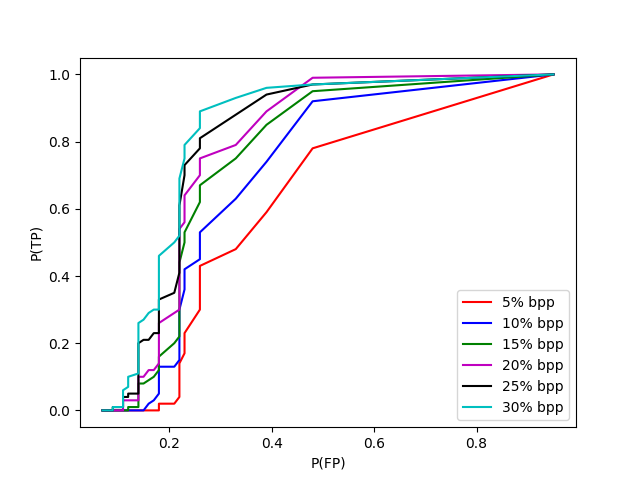
\includegraphics[width=400px, height=190px]{./images/courbe_roc.png}
\caption{\label{fig:org6dc2ee0}
Courbe ROC}
\end{figure}
\pagebreak
Afin de comparer nous avons réalisé les courbes ROC avec des insértions aléatoires

\begin{figure}[htbp]
\centering
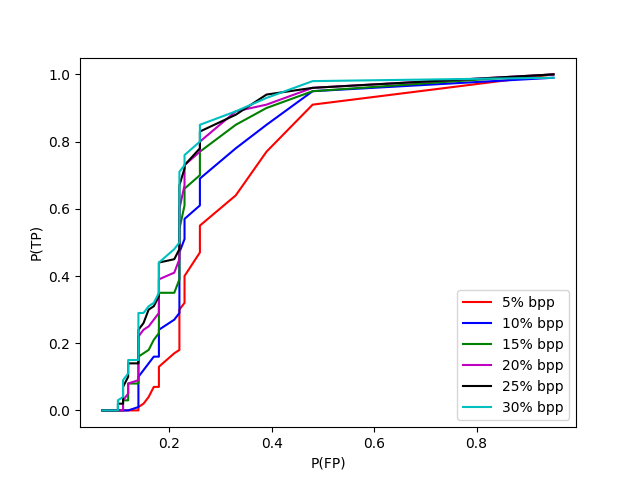
\includegraphics[width=400px, height=190px]{./images/courbe_roc_seed.png}
\caption{\label{fig:org04a80b2}
Courbe ROC avec aléatoire}
\end{figure}

Comme vous pouvez le voir les courbes sont légérement différentes.
EXPLIQUER POURQUOI
\clearpage
\section{Conclusion}

Ce travail pratique fut très intéressant et très formateur. En effet, dans un premier temps, celui-ci nous a permit
d'appréhender le langage Golang. Mais ce n'est pas tout la technique de LSB était 
une technique de dissumlation de données que nous avions rapedement vu,
mais sans jamais prendre le temps nécessaires à sa bonne comprehension. L'implementation
de notre propre version du LSB nous a permit d'assimiler entièrement son fonctionnement.


\label{sec:orgf6fc50a}

\pagebreak

\section{Annexes}
\label{sec:org831bd28}

\subsection{Compilation}
\label{sec:orge5b0aab}
Pour compiler le programme veuillez-vous assurer dans un premier temps que vous avez bien Go d'installé sur votre ordinateur et que la variable globale GOPATH possède une valeur.
Vous pouvez voir les valeurs des variables Golang avec la commande suivante.

\begin{lstlisting}[language=bash]
go env
\end{lstlisting}
\vspace{1\baselineskip}
\space
Ensuite, il faut déplacer le contenu de l'archive dans le répertoire \textbf{\$GOPATH/src/github.com/gachampiat}. 
Il faut maintenant télécharger les dépendances de notre programme pour cela tapez la commande suivante

\begin{lstlisting}[language=bash]
go get golang.org/x/image/bmp
\end{lstlisting}
\vspace{1\baselineskip}
\space
Maintenant que vous avez toutes les dépendences vous être prêt à utiliser notre programme, pour cela, vous devez le compiler
\begin{lstlisting}[language=bash]
go build go-lsb.go
\end{lstlisting}
\vspace{1\baselineskip}
\space
Après cette commande, un binaire nommé \textbf{go-lsb} devrait être créé dans votre répertoire courrant.

\subsection{Utilisation}
\label{sec:orge5b0aab}
Pour avoir une aide sur l'utilisation du programme vous pouvez simplement l'appeller sans argument, une aide
d'utilisation devrait apparaître.

\begin{lstlisting}[language=bash]
go-lsb
\end{lstlisting}
\vspace{1\baselineskip}
\space
Ci-dessous des exemples d'utilisation pour que vous puissiez bien comprendre son fonctionnement.
\vspace{1\baselineskip}
\\
\textbf{Insertion}
\vspace{1\baselineskip}
\\
Ici, nous avons une insertion simple dans une image. Le texte à inséré se trouve dans le fichier text.txt.
\begin{lstlisting}[language=bash]
go-lsb -insert image_src.bmp image_dst.bmp text.txt
\end{lstlisting}
\vspace{1\baselineskip}
\space
Si maintenant nous voulons chiffrer les données insérées il suffit de rajouter l'option key, comme ci-dessous.
\begin{lstlisting}[language=bash]
go-lsb -key MYKEY -insert image_src.bmp image_dst.bmp text.txt
\end{lstlisting}
\vspace{1\baselineskip}
\space
Enfin si nous voulons insérer les données de manières "aléatoire"
\begin{lstlisting}[language=bash]
go-lsb -key MYKEY -seed THISISMYSEED -insert image_src.bmp image_dst.bmp text.txt
\end{lstlisting}
\vspace{1\baselineskip}
\\
\textbf{Récupération}
\vspace{1\baselineskip}
\\
Après avoir vu comment insérer les données nous allons voir comment les récupérer.
Dans un premier temps, nous allons efféctuer une récupération simple.
\begin{lstlisting}[language=bash]
go-lsb -retrive image_dst.bmp
\end{lstlisting}
\vspace{1\baselineskip}
\space
Le contenu du fichier text.txt sera alors affiché sur la sortie standard. 
Ensuite comme pour l'insertion, si vous voulez dechiffrer le text, il suffit de rajouter l'option key.
\begin{lstlisting}[language=bash]
go-lsb -key MYKEY -retrive image_dst.bmp
\end{lstlisting}
\vspace{1\baselineskip}
\space
Et enfin pour finir si vous voulez récupérer le contenu qui a été inséré aléatoirement, il suffit de rajouter l'option seed.
\begin{lstlisting}[language=bash]
go-lsb -key MYKEY -seed THISISMYSEED -retrive image_dst.bmp
\end{lstlisting}
\vspace{1\baselineskip}
\\
\textbf{Détéction}
\vspace{1\baselineskip}
\\
Pour lancer la détéction sur une image, il suffit de taper la commande suivante
\begin{lstlisting}[language=bash]
go-lsb -detect image_dst.bmp
\end{lstlisting}
\subsection{Documentation}
\label{sec:orge5b0aab}
Afin d'avoir la documentation vous pouvez utiliser la commande suivante
\begin{lstlisting}[language=bash]
go doc package_name
\end{lstlisting}
\vspace{1\baselineskip}
\space
Par exemple pour voir la documentation du package lsb il suffit de taper le commande suivante
\begin{lstlisting}[language=bash]
go doc -all ./lsb
\end{lstlisting}
\clearpage
\printbibliography

\end{document}
